To further understand how coordination facts work, we present other programs that
take advantage of them.

\subsection{Belief Propagation}

Randomized and approximation algorithms can obtain significant benefits from
coordination directives because although the final program results will not be
exact, they follow important statistical properties and can be computed faster.
An examples of such programs is PageRank~\cite{Lubachevsky:1986:CAA:4904.4801}
and Loopy Belief Propagation~\cite{Gonzalez+al:aistats09paraml}, which is the
focus of this section.

Loopy Belief Propagation (LBP) is an approximate inference algorithm used in
graphical models with cycles~\cite{Murphy99loopybelief}. In its essence, LBP is
a sum-product message passing algorithm where nodes exchange messages with their
immediate neighbors and apply some computations to the messages received.

LBP is an algorithm that maps very well to the graph-based model of LM. The
original algorithm computes the belief of all nodes for several iterations with
synchronization between iterations. However, it is possible to avoid the
synchronization step, if we take advantage of the fact that LBP will converge
even when using an asynchronous approach. So, instead of computing the belief
iteratively, we keep track of all messages sent/received (and overwrite them
when we receive a new one) and recompute the belief asynchronously.
Figure~\ref{fig:coordination:bp} shows the communication patterns for our
application and Fig.~\ref{code:coordination:bp} presents the LM code for the
implementation.

\begin{figure}[h]
   \begin{center}
      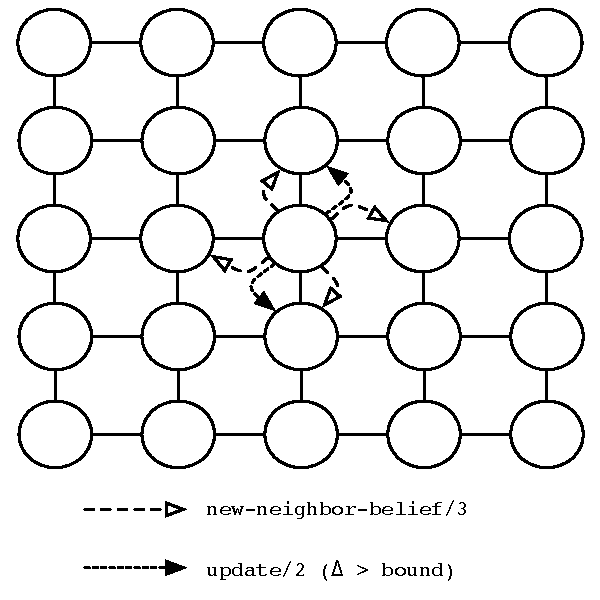
\includegraphics[width=0.3\textwidth]{figures/bp/bp.pdf}
   \end{center}
\caption{LBP: communication patterns}
\label{fig:coordination:bp}
\end{figure}

\begin{figure}[h!]
\begin{Verbatim}[numbers=left, fontsize=\codesize, commandchars=\*\{\}]
neighbor-belief(A, B, Belief),*label{line:coord:bp_first1}
new-neighbor-belief(A, B, NewBelief)
   -o neighbor-belief(A, B, NewBelief).*label{line:coord:bp_first2}

check-residual(A, Residual, B),*label{line:coord:bp_check1}
Residual > bound
   -o update(B).
check-residual(A, _, _) -o 1.*label{line:coord:bp_check2}

// update belief to be sent to one neighbor*label{line:coord:bp_iterate1}
update-messages(A, NewBelief),
!edge(A, B),
neighbor-belief-old(A, B, OldIn),
sent-neighbor-belief(A, B, OldOut),
Cavity = normalize(divide(NewBelief, OldIn)),
Convolved = normalize(convolve(global-potential, Cavity)),
OutMessage = damp(Convolved, OldOut, damping)
   -o Residual = residual(OutMessage, OldOut),
      check-residual(A, Residual, B),
      update-messages(A, NewBelief),
      new-neighbor-belief(B, A, OutMessage),
      sent-neighbor-belief(A, B, OutMessage).*label{line:coord:bp_iterate2}

update-messages(A, NewBelief) -o 1.*label{line:coord:bp_iterate_final}

// if we have two update functions, just run one of them*label{line:coord:bp_last1}
update(A), update(A) -o update(A).*label{line:coord:bp_update}

// make a copy of neighbors beliefs in order to add them up*label{line:coord:bp_update1}
update(A),
!potential(A, Potential),
belief(A, MyBelief)
   -o [custom addfloats Potential => Belief | B, Belief |*label{line:coord:bp_agg1}
         neighbor-belief(A, B, Belief) |
         neighbor-belief-old(A, B, Belief), neighbor-belief(A, B, Belief) |
         Normalized = normalizestruct(Belief),
         update-messages(A, Normalized), belief(A, Normalized)].*label{line:coord:bp_last2}*label{line:coord:bp_update2}*label{line:coord:bp_agg2}
\end{Verbatim}
\caption{LM code for the Loopy Belief Propagation problem.}
\label{code:coordination:bp}
\end{figure}

Belief values are arrays of floats and are represented by \code{belief/2} facts.
The first rule (lines~\ref{line:coord:bp_first1}-\ref{line:coord:bp_first2})
updates a given neighbor belief whenever a new belief value is received. This is
the highest priority rule since we want to update the neighbor beliefs before
doing anything else. In order to store the belief values of the neighbor nodes,
we use \code{neighbor-belief/3} facts, where the second argument is the neighbor
address and the third argument is the belief value.

The last two rules (lines~\ref{line:coord:bp_last1}-\ref{line:coord:bp_last2})
update the belief value of a node. An \code{update/1} fact starts the process.
The first rule (lines~\ref{line:coord:bp_update}) simply consumes redundant
\code{update/1} facts and the second rule
(lines~\ref{line:coord:bp_update1}-\ref{line:coord:bp_update2}) performs the
belief update by aggregating all the neighbor belief values. The aggregate in
lines~\ref{line:coord:bp_agg1}-\ref{line:coord:bp_agg2} also derives copies of
the neighbors beliefs that need to be consumed in order to compute the belief
value that is going to be sent to the target neighbor. The aggregate uses a
custom accumulator that takes two arrays and adds the floating point numbers at
each index of the array. The rule in
lines~\ref{line:coord:bp_iterate1}-\ref{line:coord:bp_iterate2} iterates through
the neighbor belief values and sends new belief values by performing the
appropriate computations on the new belief value of the current node and on the
belief value sent previously.  Once the facts \code{neighbor-belief-old} are
fully consumed, the rule in line~\ref{line:coord:bp_iterate_final} is fired in
order to consume \code{update-messages}.

For each neighbor update, we also check in
lines~\ref{line:coord:bp_check1}-\ref{line:coord:bp_check2} if the change in
belief values is greater than \code{bound} (a program constant) and then force
the neighbor nodes to update their belief values by deriving \code{update(B)}.
This allows neighbor nodes to use updated neighbor values and recompute their
own belief values using better information. The computation of belief values
will then start to converge to their true belief values, independently of the
node scheduling used. However, if we prioritize nodes that receive new neighbor
belief values with a larger \code{Residual} then we will converge faster.
Figure~\ref{code:coordination:improved_bp} shows the fourth rule modified with
\code{add-priority} in order to increase to priority of neighbor nodes when the
source node has large changes in its belief value.

\begin{figure}[h!]
\begin{Verbatim}[numbers=left,commandchars=\\\{\},fontsize=\codesize]
// update belief to be sent to one neighbor
update-messages(A, NewBelief),
!edge(A, B),
neighbor-belief-old(A, B, OldIn),
sent-neighbor-belief(A, B, OldOut),
Cavity = normalize(divide(NewBelief, OldIn)),
Convolved = normalize(convolve(global-potential, Cavity)),
OutMessage = damp(Convolved, OldOut, damping)
   -o Residual = residual(OutMessage, OldOut),
      \underline{add-priority(B, Residual)},
      check-residual(A, Residual, B),
      update-messages(A, NewBelief),
      new-neighbor-belief(B, A, OutMessage),
      sent-neighbor-belief(A, B, OutMessage).
\end{Verbatim}
\caption{Updating the BP program to use priorities.}
\label{code:coordination:improved_bp}
\end{figure}

\subsection{N Queens}
The N-Queens puzzle is the problem of placing N chess queens on an NxN
chessboard so that no pair of two queens attack each other~\cite{8queens}. The
specific challenge of finding all the distinct solutions to this problem is a
good benchmark in designing parallel algorithms.  Most popular parallel
implementations of the N-Queens problem distribute the search space of the
problem by assigning incomplete boards as tasks to threads.  Our approach is
unusual since the squares of the board as the tasks of program.
Figure~\ref{code:coordination:nqueens} presents our solution.

N Queens nodes are the squares of the chessboard and each square can communicate
with other 4 squares: the adjacent right and the adjacent left on the same row,
and the first non-diagonal square to the right and to the left on the row below.
To represent a partial/valid board state, we use a list of integers, where each
pair of integers represents a coordinate in which a queen is placed. For example
$[1, 2, 0, 0]$ means that a queen is placed in square $(0, 0)$ and another in
square $(1, 2)$. At any given time, many partial states can be using the same
squares.  Each square can also have many states at the same time.

\begin{figure}[ht!]
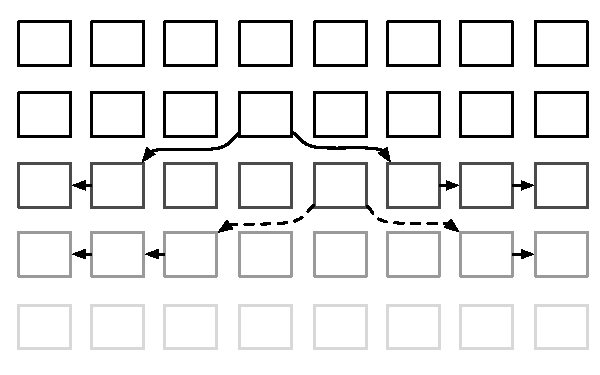
\includegraphics[width=0.4\textwidth]{figures/coordination/nqueens.pdf}
\caption{Concurrent propagation of N-Queens states.}
\label{coordination:fig:nqueens}
\end{figure}

An empty state is instantiated in the top-left square
(line~\ref{line:coord:queens_axiom}) and is then propagated to all squares in
the same row (rule in
lines~\ref{line:coord:queens_propr1}-\ref{line:coord:queens_propr2}). Once a
square $S$ receives a new state $L$, it checks if $S$ can be incorporated into
$L$. For that, it checks if there is no queen on $S$'s column (rules in lines
\ref{line:coord:queens_col1}-\ref{line:coord:queens_col2}), if there is no queen
on $S$'s left diagonal (rules in
lines~\ref{line:coord:queens_ldiag1}-\ref{line:coord:queens_ldiag2}) and if
there is no queen on $S$'s right diagonal (rules in
lines~\ref{line:coord:queens_rdiag1}-\ref{line:coord:queens_rdiag2}).

If there is any conflict, we do not derive anything and for that we use the
language expression \code{1}
(lines~\ref{line:coord:queens_empty1},~\ref{line:coord:queens_empty2}
and~\ref{line:coord:queens_empty3}). If there are no conflicts, this means that
it is possible to add a queen to the current state
(line~\ref{line:coord:queens_add}). The fact \code{send-down/2} is used to
either complete the computation of a valid state
(lines~\ref{line:coord:queens_complete1}-\ref{line:coord:queens_complete2}) or
to propagate the state to the row below
(lines~\ref{line:coord:queens_down1}-\ref{line:coord:queens_down2}) as shown in
Fig.~\ref{coordination:fig:nqueens}.

Since computation goes from the top row to the bottom row, not all static
placements of nodes to threads will perform equally well. This is especially
true because the bottom rows tend to perform the most work.  The best placement
is then to split the board vertically with axiom \code{set-thread(A, vertical(X,
Y))} so each thread gets the same number of columns, where \code{X} and \code{Y}
are the coordinates of a particular square. Our experiments show that, on a
shared memory system, it does not matter much if we start with a bad placement
since node stealing overcomes those issues by load balancing dynamically.
However, the N Queens program incrementally builds and shares lists representing
valid board states that are transmitted from top to bottom. In order to improve
memory locality we should then manipulate board states that share a significant
number of elements because each board state needs to be iterated before being
extended with a new position. To accomplish this, we used the coordination fact
\code{set-default-priority(A, X)} to experiment with two configurations:
\code{Top}, where top rows are prioritized; and \code{Bottom}, where squares
closer to the bottom are computed first. We also decided to optionally pin nodes
to threads, as mentioned earlier, to see if memory locality affects the
multi-threaded performance of the program.

%% XXX results
\begin{figure}[h!]
\begin{Verbatim}[numbers=left,fontsize=\scriptsize,commandchars=\*\#\&]
type list int state.
type left(node, node).  type right(node, node).
type down-left(node, node).  type down-right(node, node).
type coord(node, int, int).
type linear propagate-left(node, state).
type linear propagate-right(node, state).
type linear test-y(node, int, state, state).
type linear test-diag-left(node, int, int, state, state).
type linear test-diag-right(node, int, int, state, state).
type linear send-down(node, state).
type linear new-state(node, state).
type linear final-state(node, state).

propagate-right(@0, []).*label#line:coord:queens_axiom&

propagate-left(A, State)
  -o {L | !left(A, L), L <> A | propagate-left(L, State)}, new-state(A, State).
propagate-right(A, State)*label#line:coord:queens_propr1&
  -o {R | !right(A, R), R <> A | propagate-right(R, State)}, new-state(A, State).*label#line:coord:queens_propr2&

new-state(A, State), !coord(A, X, Y) -o test-y(A, Y, State, State).

// check if there is no queen on the same column*label#line:coord:queens_col1&
test-y(A, Y, [], State), !coord(A, OX, OY)
  -o test-diag-left(A, OX - 1, OY - 1, State, State).
test-y(A, Y, [X, Y1 | RestState], State), Y = Y1
  -o 1. // fail*label#line:coord:queens_empty1&
test-y(A, Y, [X, Y1 | RestState], State), Y <> Y1
  -o test-y(A, Y, RestState, State).*label#line:coord:queens_col2&

// check if there is no queen on the left diagonal*label#line:coord:queens_ldiag1&
test-diag-left(A, X, Y, _, State), X < 0 || Y < 0, !coord(A, OX, OY)
  -o test-diag-right(A, OX - 1, OY + 1, State, State).
test-diag-left(A, X, Y, [X1, Y1 | RestState], State), X = X1, Y = Y1
  -o 1. // fail*label#line:coord:queens_empty2&
test-diag-left(A, X, Y, [X1, Y1 | RestState], State), X <> X1 || Y <> Y1
  -o test-diag-left(A, X - 1, Y - 1, RestState, State).*label#line:coord:queens_ldiag2&

// check if there is no queen on the right diagonal*label#line:coord:queens_rdiag1&
test-diag-right(A, X, Y, [], State), X < 0 || Y >= size, !coord(A, OX, OY)
  -o send-down(A, [OX, OY | State]). // add new queen*label#line:coord:queens_add&
test-diag-right(A, X, Y, [X1, Y1 | RestState], State), X = X1, Y = Y1
  -o 1. // fail*label#line:coord:queens_empty3&
test-diag-right(A, X, Y, [X1, Y1 | RestState], State), X <> X1 || Y <> Y1
  -o test-diag-right(A, X - 1, Y + 1, RestState, State).*label#line:coord:queens_rdiag2&

send-down(A, State), !coord(A, size - 1, _)*label#line:coord:queens_complete1&
  -o final-state(A, State).*label#line:coord:queens_complete2&
send-down(A, State), !coord(A, CX, _), CX <> size - 1*label#line:coord:queens_down1&
  -o {B | !down-right(A, B), B <> A | propagate-right(B, State)},
     {B | !down-left(A, B), B <> A | propagate-left(B, State)}.*label#line:coord:queens_down2&
\end{Verbatim}
  \caption{N-Queens problem solved in LM.}
  \label{code:coordination:nqueens}
\end{figure}


\subsubsection{Proof Of Correctness}

\begin{lemma}[test-y lemma]

If \code{test-y(A, Y, State, OriginalState)} then either $\exists_{x'}. {(x',
y) \in \mathtt{State}}$ and \code{test-y} is consumed or
\code{test-diag-left(A, OX - 1, OY - 1, OriginalState, OriginalState)}, where
\code{OX} and \code{OY} are the coordinates of the square.

\end{lemma}
\begin{proof}
Induction on the size of \code{State}.

First rule: immediately the second conclusion.

Second rule: immediately the third conclusion.

Third rule: by induction.
\end{proof}

\begin{lemma}[test-diag-left lemma]
If \code{test-diag-left(A, X, Y, State, OriginalState)} then either $\exists_{x', y'}. {(x', y') \in \mathtt{State}}$, where $x = x' - a$ and $y' = y - a$, where $a$ is positive or $0$ and \code{test-diag-left} is consumed or \code{test-diag-right(A, OX - 1, OY + 1, OriginalState, OriginalState)}, where \code{OX} and \code{OY} are the coordinates of the square.
\end{lemma}
\begin{proof}
Induction on the size of \code{State}.

First rule: immediately the second conclusion.

Second rule: immediately the first conclusion.

Third rule: by induction.
\end{proof}

\begin{lemma}[test-diag-right lemma]
If \code{test-diag-right(A, X, Y, State, OriginalState)} then either $\exists_{x', y'}. {(x', y') \in \mathtt{State}}$, where $x = x' - a$ and $y' = y + a$, where $a$ is positive or $0$ and \code{test-diag-right} is consumed or \code{send-down(A, [(OX, OY) | OriginalState])}, where \code{OX} and \code{OY} are the coordinates of the square.
\end{lemma}
\begin{proof}
Induction on the size of \code{State}.

First rule: immediately the second conclusion.

Second rule: immediately the first conclusion.

Third rule: by induction.
\end{proof}

\begin{theorem}[State validation]
If \code{test-y(A, OY, State, State)} then either everything is consumed or \code{send-down(A, [(OX, OY) | State])} is derived, where \code{OX} and \code{OY} are the coordinates of the square and are a valid addition to the \code{State}.
\end{theorem}
\begin{proof}
Use the previous three lemmas.
\end{proof}

\begin{lemma}[Propagate left lemma]
If \code{propagate-left(A, State)} then every cell to the left, including \code{A} will derive \code{new-state(A, State)}.
\end{lemma}
\begin{proof}
By induction on the number of cells to the left of \code{A}. The only rule that uses \code{propagate-left/2} will prove the lemma.
\end{proof}

\begin{lemma}[Propagate right lemma]
If \code{propagate-right(A, State)} then every cell to the right, including \code{A} will derive \code{new-state(A, State)}.
\end{lemma}
\begin{proof}
By induction on the number of cells to the right of \code{A}. The only rule that uses \code{propagate-right/2} will prove the lemma.
\end{proof}

\begin{theorem}[States theorem]
For a given row, we will compute several \code{send-down(A, State)} facts that represent valid configurations that include that row and the rows above.
\end{theorem}
\begin{proof}
By induction on the number of rows.

For row 0, we use the axiom \code{propagate-right(@0, [])}, that will be propagated to all nodes in row 0. By using the state validation theorem, we know that every node will derive \code{send-down(A, [(X, Y)])}, all valid configurations.


By induction, we know that row $X'$ has derived every \code{send-down/2} possible. Such facts will be sent downwards to row $X = X' + 1$ using the last rule in the program, deriving \code{propagate-right} or \code{propagate-left} that will derive \code{new-state} at each right or left cell. We do not derive anything at the cell below or the ones to the sides since they would not be valid. Using the \code{new-state} fact, we get a \code{test-y} fact that will be checked using the state validation theorem, filtering all new valid configurations and deriving \code{send-down/2}.
\end{proof}

\clearpage


\subsection{Heat Transfer}

In the Heat Transfer~(HT) algorithm, we have a graph where heat values are
exchanged between nodes. The program stops when the new heat values $H_i$
differ only a small $\epsilon$ from the old values $H_{i-1}$, where $\delta =
|H_i - H_{i-1}| \le \epsilon$. The algorithm works asynchronously, i.e., heat
values are updated using information as it arrives from neighboring nodes. This
increases concurrency since nodes do not need to synchronize between
iterations.

Figure~\ref{code:coord:ht} shows the HT rules that send new heat values to
neighbor nodes. In the first rule we added \code{add-priority} action fact to
increase the priority of the neighbor nodes for the case when the current node has a large
$\delta$. The idea is to prioritize the computation of heat values of nodes
(using \code{update}) that have a neighbor that changed significantly. Multiple
\code{add-priority} facts will increase the priority of a node so that nodes
with multiple large deltas will have more priority.

\begin{figure}[h!]
\begin{Verbatim}[numbers=left,fontsize=\codesize,commandchars=\\\[\]]
new-heat(A, New, Old),
Delta = fabs(New - Old),
Delta > epsilon
   -o {B | !edge(A, B) |
         new-neighbor-heat(B, A, New),
         update(B), \underline[add-priority(B, Delta)]}.

new-heat(A, New, Old)
fabs(New - Old) <= epsilon
   -o {B | !edge(A, B) |
         new-neighbor-heat(B, A, New)}.
\end{Verbatim}
  \caption{Coordination code for the Heat Transfer program.}
  \label{code:coord:ht}
\end{figure}

\iffalse
Fig.~\ref{results:ht} presents the scalability results for the regular
and coordinated version. The dataset used is a square grid with an inner square
with high heat nodes. Comparing the coordinated version with the regular
version, with 1 thread there is a 50\% reduction in run time, while
for 16 threads there is, on average, a 25\% reduction.
\fi

To further improve locality, we can split the second rule to avoid sending small
$\delta$ values if the target node is in another thread
(Fig.~\ref{code:coord:ht_better}). We use \code{thread-id} to retrieve the
thread \code{T} of the node \code{A} and match the \code{thread-id} of each
neighbor \code{B} against \code{T}. The comprehension in
lines~\ref{line:coord:ht_better_comp1}-\ref{line:coord:ht_better_comp2} only
generates \code{new-neighbor-heat} facts if \code{B} is in the same thread.

\iffalse
The \textbf{C/Local} line in
Fig.~\ref{results:ht} shows that this performs best.  However, this comes at
the price of increased errors in the computed heat values.
\fi

\begin{figure}[h!]
\begin{Verbatim}[numbers=left,fontsize=\codesize,commandchars=\\\[\]]
new-heat(A, New, Old)
fabs(New - Old) <= epsilon,
\underline[thread-id(A, T)]
   -o {B, T | !edge(A, B), \underline[thread-id(B, T)] |\label[line:coord:ht_better_comp1]
         new-neighbor-heat(B, A, New), \underline[thread-id(B, T)]},\label[line:coord:ht_better_comp2]
      \underline[thread-id(A, T)].
\end{Verbatim}

  \caption{To improve locality, we add an extra constraint to the second rule to
     avoid sending small $\delta$ values if the target node is in another thread.}
  \label{code:coord:ht_better}
\end{figure}

\subsection{MiniMax}
The MiniMax algorithm is a decision rule algorithm for minimizing the possible
loss for a worst case (maximum loss) scenario in a zero sum game for 2 (or more)
players who play in turns.

The algorithm builds a game tree, where each tree node represents a game state
and the children represent the possible game moves that can be made by either
player 1 or player 2.  An evaluation function is used to compute the score of
the game for each leaf of the tree. A node is a leaf when the game state can no
longer be expanded. Finally, the algorithm recursively minimizes or maximizes
the scores of each node. To select the best move for player 1, the algorithm
picks the move maximized at the root node.

Figure~\ref{code:coord:minimax} shows LM's code for the MiniMax program using
coordination facts. The program starts with a root node (with the initial game state) that
is expanded with the available moves at each level. The graph of the program is
dynamic since nodes are created and then deleted once they are no longer
needed. The latter happens when the leaf scores are computed or when a node
fully minimizes or maximizes the children scores. When the program ends, only
the root node has facts in its database.

The first two rules in
lines~\ref{line:coord:minimax_play1}-\ref{line:coord:minimax_play2} check if the
current game is final, namely, if a player has won or the game drew: the first
rule generates the score for the final state while the second expands the game
state by generating all the possible plays for player \code{NextPlayer}.

The expansion rules create the children for the current node and are
implemented in
lines~\ref{line:coord:minimax_expand1}-\ref{line:coord:minimax_expand2}. The
first two rules create either a \code{maximize} or \code{minimize} fact that
will either maximize or minimize the scores of the children nodes.  The third
and fourth expansion rules simulate a player move and, for that, create a new
node \code{B} using the \code{exists} language construct. We link \code{B} with
\code{A} using \code{parent(B, A)} and kickstart the recursive expansion of node
\code{B} by deriving a \code{play} fact. Finally, the rule in
lines~\ref{line:coord:minimax_expand11}-\ref{line:coord:minimax_expand2} is for
the case when the current player cannot play in the current game position. The
full proof of correctness is presented in
Appendix~\ref{appendix:proofs:minimax}.

\iffalse
\begin{wrapfigure}{r}{0.4\textwidth}
   \begin{center}
      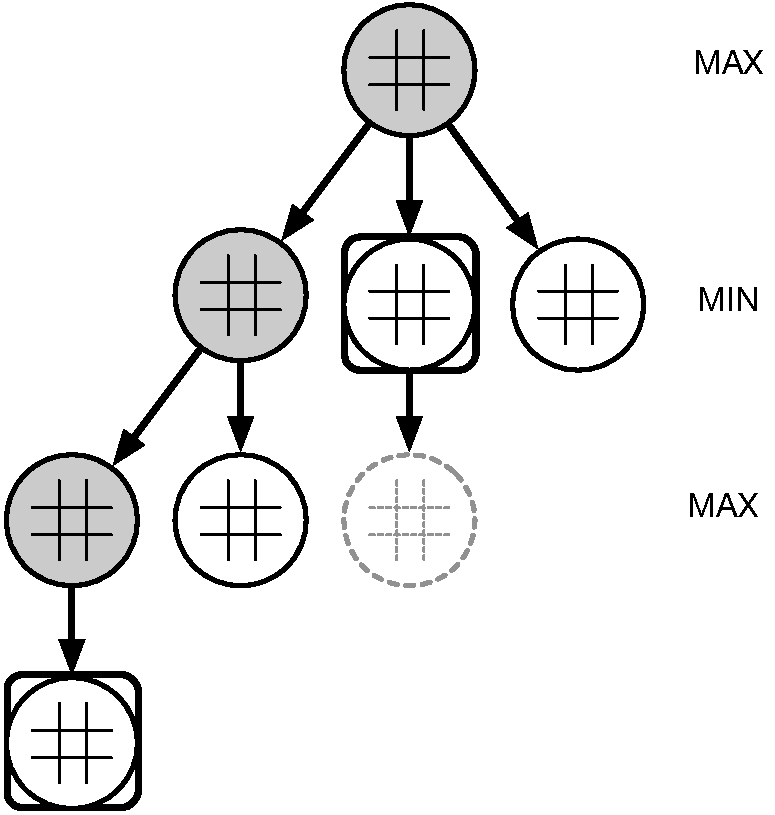
\includegraphics[width=0.9\linewidth]{figures/coordination/minimax_tree}
   \end{center}
   \caption{Expanding the MiniMax tree using coordination. By prioritizing
      deeper nodes, threads are forced to expand the tree using a depth-first
      approach, which is superior since there is no need to expand the whole
      tree before computing the node scores.}
   \label{fig:coord:minimax}
\end{wrapfigure}
\fi

As noted in Section~\ref{sec:coord:fifo}, LM's default scheduler uses a FIFO
approach, which results in a breadth-first expansion of the MiniMax tree. This
results in $\mathcal{O}(n)$ space complexity, where $n$ is the number of nodes
in the tree, since the tree must be fully expanded before the scores at the
leaves are actually computed.  With coordination, we set the priority of a node
to be its depth (lines~\ref{line:coord:minimax_coord1} and
\ref{line:coord:minimax_coord2}) so that the tree is expanded in a depth-first
fashion, leading to $\mathcal{O}(d t)$ memory complexity, where $d$ is the depth
of the tree and $t$ is the number of threads. Since threads prioritize deeper
nodes, the scores of the first leaves are immediately computed and then sent to
the parent node. At this point, the leaves are deleted and reused for other
nodes in the tree, resulting in minimal memory usage.  As an example, consider a
system with 2 threads, $T_1$ and $T_2$, where $T_1$ first expands the root node
and then the first child. Since $T_2$ is idle, it steals half of the root's
children nodes and starts expanding one of the nodes in a depth-first fashion.

\begin{figure}[ht]
\begin{Verbatim}[numbers=left,commandchars=\\\{\},fontsize=\scriptsize]
type list int game.\hfill// Type declaration
type linear parent(node, node).\hfill// Predicate declaration
type linear score(node, int, int).
type linear new-score(node, int, int).
type linear minimize(node, int, int, int).
type linear maximize(node, int, int, int).
type linear expand(node, game FirstPart, game SecondPart, int Descendants, int Player, int Play, int Depth).
type linear play(node, game Game, int Player, int Play, int Depth).

const root-player = 1. const initial-game = [...].\hfill// Constant declaration: player and initial game state
fun next(P : int) : int = if P = 1 then 2 else 1 end.\hfill// Function declaration: select next player

play(A, Game, NextPlayer, LastPlay, Depth),\label{line:coord:minimax_play1}\label{line:coord:minimax_play11}\hfill// Rule 1: ending game state
Score = minimax_score(Game, NextPlayer, root-player), Score > 0
   -o score(A, Score, LastPlay).\label{line:coord:minimax_play12}

play(A, Game, NextPlayer, LastPlay, Depth),\label{line:coord:minimax_play21}\hfill// Rule 2: expand state
0 = minimax_score(Game, NextPlayer, root-player)
   -o expand(A, [], Game, 0, NextPlayer, LastPlay, Depth).\label{line:coord:minimax_play2}\label{line:coord:minimax_play22}

expand(A, Game, [], N, Player, Play, \underline{Depth}), Player = root-player\label{line:coord:minimax_expand1}\label{line:coord:minimax_rule11}\hfill// Rule 3: maximize node
   -o maximize(A, N, -00, 0).\label{line:coord:minimax_rule12}

expand(A, Game, [], N, Player, Play, \underline{Depth}), Player <> root-player\label{line:coord:minimax_rule21}\hfill// Rule 4: minimize node
   -o minimize(A, N, +00, 0).\label{line:coord:minimax_rule22}

expand(A, First, [0 | Xs], N, Player, Play, \underline{Depth}), Depth >= 5\label{line:coord:minimax_rule31}\hfill// Rule 5: create static child node
   -o exists B. (\underline{set-static(B)},\label{line:coord:minimax_coord1}
       \underline{set-default-priority(B, float(Depth + 1))},\label{line:coord:minimax_coord2}
       play(B, Game ++ [P | Xs], next(P), length(First), \underline{Depth + 1}), parent(B, A).
       expand(A, First ++ [0], Xs, N + 1, Player, Play, \underline{Depth})).\label{line:coord:minimax_rule32}

expand(A, First, [0 | Xs], N, Player, Play, \underline{Depth}), Depth < 5\label{line:coord:minimax_rule41}\hfill// Rule 6: create child node
  -o exists B. (\underline{set-default-priority(B, float(Depth + 1))},\label{line:coord:minimax_coord3}
       play(B, Game ++ [P | Xs], next(P), length(First), \underline{Depth + 1}), parent(B, A),
       expand(A, First ++ [0], Xs, N + 1, Player, Play, \underline{Depth})).\label{line:coord:minimax_rule42}

expand(A, First, [C | Xs], N, Player, Play, \underline{Depth}) C <> 0\label{line:coord:minimax_expand11}\label{line:coord:minimax_rule51}\hfill// Rule 7: next game play
  -o expand(A, First ++ [C], Xs, N, Player, Play, \underline{Depth}).\label{line:coord:minimax_expand2}\label{line:coord:minimax_rule52}

score(A, Score, BestPlay), parent(A, B) -o new-score(B, Score, BestPlay).\label{line:coord:minimax_new}\hfill// Rule 8: sending score to parent node

new-score(A, Score, Play), minimize(A, N, Current, BestPlay), Current > Score\label{line:coord:minimax_minimize1}\hfill// Rule 9: keep current score
   -o minimize(A, N - 1, Score, Play).

new-score(A, Score, Play), minimize(A, N, Current, BestPlay), Current <= Score\hfill// Rule 10: select new best
   -o minimize(A, N - 1, Current, BestPlay).

minimize(A, 0, Score, BestPlay) -o score(A, Score, BestPlay).\label{line:coord:minimax_minimize2}// Rule 11: score minimized

new-score(A, Score, Play), maximize(A, N, Current, BestPlay), Current < Score\label{line:coord:minimax_maximize1}\label{line:coord:minimax_maximize_rule11}\hfill// Rule 12: keep current score
   -o maximize(A, N - 1, Score, Play).\label{line:coord:minimax_maximize_rule12}

new-score(A, Score, Play), minimize(A, N, Current, BestPlay), Current >= Score\label{line:coord:minimax_maximize_rule21}\hfill// Rule 13: select new best
   -o maximize(A, N - 1, Current, BestPlay).\label{line:coord:minimax_maximize_rule22}

maximize(A, 0, Score, BestPlay) -o score(A, Score, BestPlay).\label{line:coord:minimax_maximize2}\hfill// Rule 14: score maximized

play(@0, initial-game, root-player, 0, 1).\label{line:coord:minimax_axiom}\hfill// Initial fact
\end{Verbatim}
\caption{LM code for the MiniMax program.}
\label{code:coord:minimax}
\end{figure}

We also take advantage of memory locality by using \code{set-static}
(line~\ref{line:coord:minimax_coord2}), so that nodes after a certain level are
   not stolen by other threads. While this is not critical for performance in
   shared memory systems where node stealing is fairly efficient, we expect that
   such coordination to be critical in distributed systems.

The rest of the program contains rules for maximizing and minimizing scores
(lines~\ref{line:coord:minimax_minimize1}-\ref{line:coord:minimax_maximize2}),
through the retraction of \code{new-score} incoming facts.

\begin{figure}[ht]
   \begin{center}
      \begin{tabular}{c | c || c c | c c | c c} \hline
	 \multirow{2}{*}{\textbf{Size}} & \multirow{2}{*}{\textbf{Threads}} & \multicolumn{2}{c|}{\textbf{Average}} & \multicolumn{2}{c|}{\textbf{Final}} & \multicolumn{2}{c}{\textbf{\# Malloc}}\\
	 & & Regular & Coord & Regular & Coord & Regular & Coord\\ \hline \hline
\multirow{7}{*}{Small}  & 1 &  1794.8MB & 38KB &  33KB & 33KB &  42 & 11\\
 & 2 &  869.4MB & 35KB &  64KB & 65KB &  80 & 22\\
 & 4 &  436.2MB & 34KB &  128KB & 129KB &  152 & 44\\
 & 8 &  198.6MB & 32KB &  254KB & 258KB &  284 & 88\\
 & 16 &  65.3MB & 33KB &  508KB & 514KB &  513 & 172\\
 & 24 &  40.5MB & 32KB &  761KB & 770KB &  742 & 256\\
 & 32 &  24.4MB & 32KB &  1014KB & 1022KB &  953 & 335\\
\hline
\multirow{7}{*}{Big}  & 1 &  14.5GB & 43KB &  33KB & 33KB &  48 & 12\\
 & 2 &  7.2GB & 35KB &  64KB & 65KB &  92 & 24\\
 & 4 &  2.4GB & 36KB &  128KB & 130KB &  172 & 45\\
 & 8 &  1748.3MB & 33KB &  254KB & 258KB &  331 & 89\\
 & 16 &  665.10MB & 34KB &  508KB & 515KB &  620 & 177\\
 & 24 &  271.3MB & 35KB &  761KB & 771KB &  871 & 265\\
 & 32 &  193.5MB & 34KB &  1014KB & 1027KB &  1123 & 353\\
\hline
\end{tabular}

   \end{center}

   \caption{Comparing the memory usage of the regular and coordinated MiniMax
   programs.}
   \label{results:memory_minmax}
\end{figure}

In Table~\ref{results:memory_minmax} we compare the memory usage of the
coordinated MiniMax program against the regular MiniMax program. The
\textbf{Average} column presents the average memory usage during the lifetime of
the program, the \textbf{Final} indicates the amount of memory used at the end
of the program, while the \textbf{\# Malloc} column represents the number of
calls made to the \code{malloc} function by the threaded allocator. The
coordinated version uses significantly less memory than the regular version. As
the number of the threads increases, the average memory usage of the regular
version decreases because there are more threads that are able to complete
different parts of the tree at the same time. The same thing happens for the
coordinated version, but at a much smaller scale since threads are exploring the
tree in a depth-first fashion. Finally, as expected, there is also a large
reduction in the number of \code{malloc}'s called by the threaded allocator in
the coordinated version.

The run time and scalability results are presented in
Fig.~\ref{fig:coordination:results_minmax}. There is a clear performance
improvement when coordinating the MiniMax program due to the low memory usage.
The Big dataset needs only 5 threads to reach the performance of the
sequential C++ program and, when using 32 threads, the LM program is more than
four times faster than the C++ version. The use of coordination facts allows us
to improve the execution of this declarative program and make it run
significantly faster than it would be otherwise.

\begin{figure}[]
        \centering
        \begin{subfigure}[b]{\plotsize\textwidth}
           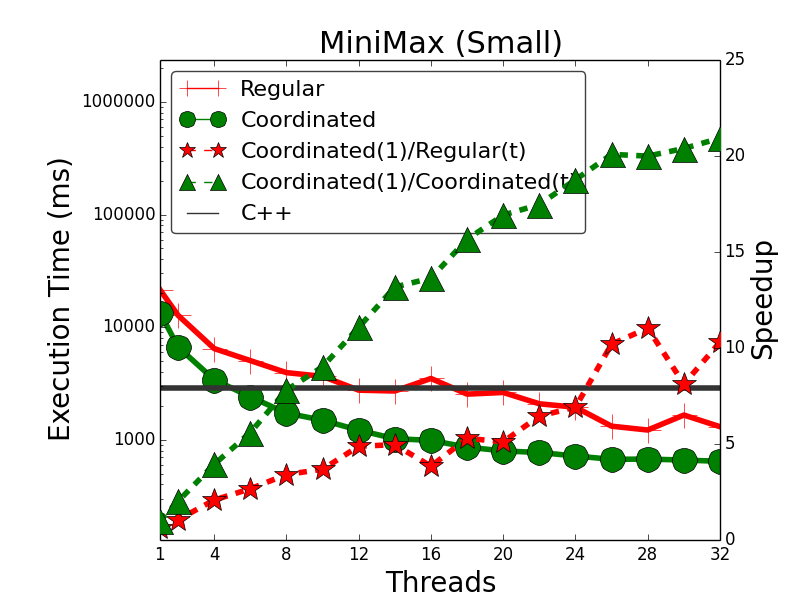
\includegraphics[width=\textwidth]{experiments/coordination/cmp-min-max-tictactoe-small.png}
           \label{fig:coordination:coord_minimax_small}
        \end{subfigure}
        ~
        \begin{subfigure}[b]{\plotsize\textwidth}
           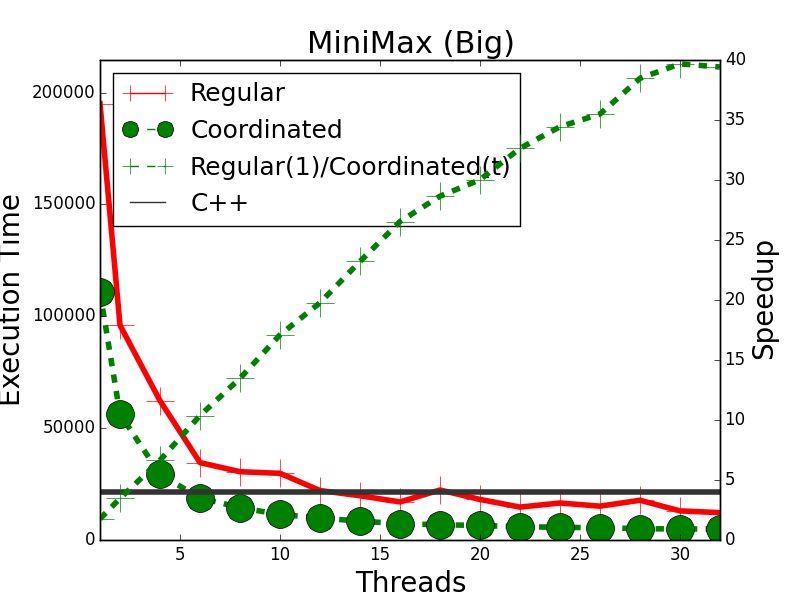
\includegraphics[width=\textwidth]{experiments/coordination/cmp-min-max-tictactoe-big.png}
           \label{fig:coordination:coord_minimax_big}
        \end{subfigure} \\

        \caption{Scalability for the MiniMax program when using coordination.}

        \label{fig:coordination:results_minmax}
\end{figure}

\clearpage

